\documentclass[preprint,12pt]{elsarticle}

\usepackage{amsmath,amssymb,amsthm}
\usepackage[T1]{fontenc}
\usepackage{lmodern}
\usepackage{microtype}

\journal{Applied Mathematics Letters}

\makeatletter
% Match the journal-style e-mail footnote shown in the target example.
\@ifundefined{patchcmd}{}{%
    \patchcmd{\printFirstPageNotes}{Email address:}{E-mail address:}{}{}%
    \patchcmd{\printFirstPageNotes}{Email addresses:}{E-mail addresses:}{}{}%
}
\newcommand{\eadauthorname}[1]{\@eadauthor={#1}}
\makeatother

\newtheorem{lemma}{Lemma}
\newtheorem{theorem}{Theorem}
\newtheorem{remark}{Remark}

\DeclareMathOperator*{\argmin}{arg\,min}
\renewcommand{\qedsymbol}{$\blacksquare$}

\begin{document}

\begin{frontmatter}

\title{Finite-Time Convergence of Competitive Graph Recoloring via Discrete Lyapunov Functions}

\author[vitap]{Ranjan Veerabhadraswamy}
\eadauthorname{R. Veerabhadraswamy}
\ead{ranjanvswamyjnv2005@gmail.com}

\author[vitap]{Ajith Jubilson Emerson\corref{cor1}}
\eadauthorname{A.J. Emerson}
\ead{ajith.jubilson@vitap.ac.in}
\cortext[cor1]{Corresponding author.}

\affiliation[vitap]{
    organization={School of Computer Science and Engineering, Vellore Institute of Technology (VIT-AP)},
    state={Andhra Pradesh},
    country={India}
}

\begin{abstract}
We study an asynchronous competitive recoloring process on a finite graph, in
which each active vertex selfishly changes color only when doing so strictly
reduces the number of same-colored neighbors. Although globally minimizing
monochromatic edges is equivalent to a MAX-$k$-CUT objective and is NP-hard in
general, the local dynamics admit a simple exact potential. We prove that every
accepted recoloring decreases the number of monochromatic edges by exactly the
local improvement, and therefore the process reaches a pure Nash equilibrium in
at most $|E|$ accepted recolorings. Simulations on sparse Erd\H{o}s--R\'enyi and
Barab\'asi--Albert graphs support the deterministic bound and show substantially
faster average-case convergence.
\end{abstract}

\begin{keyword}
graph coloring \sep best-response dynamics \sep potential game \sep discrete
Lyapunov function \sep MAX-$k$-CUT
\end{keyword}

\end{frontmatter}

\section{Introduction}

Graph recoloring under local incentives appears in distributed coordination,
interference avoidance, and networked resource assignment
\cite{kuhn2006,panagopoulou2008}. In such settings, a natural objective is to
reduce monochromatic edges, but the corresponding global optimization problem
is computationally difficult: minimizing monochromatic edges is equivalent to
maximizing bichromatic edges, i.e., to the MAX-$k$-CUT objective, which is
NP-hard in general \cite{garey1979,frieze1997}. This motivates the analysis of
distributed local heuristics whose behavior can be certified without solving
the global problem.

The game-theoretic view is equally natural. Each vertex is a player, each color
is an action, and each player seeks to reduce its local conflict cost. Pure Nash
equilibria and potential methods are classical tools for such local incentive
systems \cite{nash1951,rosenthal1973,monderer1996}.
The specific rule studied here is a strict best-response recoloring dynamics.
The main observation is that the number of monochromatic edges is an exact
discrete Lyapunov function, in the spirit of potential-based convergence
arguments for networked dynamics \cite{hopfield1982,apt2012}. Consequently,
selfish local updates cannot cycle and must reach a locally stable coloring
after at most $|E|$ accepted moves.

\section{Model}

Let $G=(V,E)$ be a finite undirected graph, with $n=|V|$ vertices and $m=|E|$
edges. Let $C=\{1,2,\ldots,k\}$ be a finite color set. A configuration is
denoted by
\[
    c=(c_i)_{i\in V}\in C^V,
\]
where $c_i$ is the color assigned to vertex $i$. For $i\in V$, let
$N(i)=\{j\in V:\{i,j\}\in E\}$ be its neighborhood. The local conflict cost of
vertex $i$ is
\[
    d_i(c_i,c_{-i})
    =
    \sum_{j\in N(i)} \mathbf{1}\{c_i=c_j\},
\]
where $c_{-i}$ denotes the colors of all vertices except $i$. Equivalently, if
the colors of the other vertices are fixed, then for any $\gamma\in C$,
\[
    d_i(\gamma,c_{-i})
    =
    \sum_{j\in N(i)} \mathbf{1}\{\gamma=c_j\}.
\]

The dynamics are asynchronous. At each activation, a single vertex $i$ is
selected. If there exists a color that strictly reduces its local conflict
cost, vertex $i$ changes to a best-response color
\[
    c_i^+ \in \argmin_{\gamma\in C} d_i(\gamma,c_{-i}),
\]
and the update is accepted only when
\[
    d_i(c_i^+,c_{-i}) < d_i(c_i,c_{-i}).
\]
Otherwise the configuration is unchanged. In what follows, a \emph{step} means
one accepted recoloring.

Define the global conflict potential
\[
    \Phi(c)
    =
    \sum_{\{u,v\}\in E} \mathbf{1}\{c_u=c_v\}
    =
    \frac12 \sum_{i\in V} d_i(c_i,c_{-i}).
\]
Thus $\Phi(c)$ is exactly the number of monochromatic edges.

\section{Finite convergence}

\begin{lemma}[Exact potential drop]
Let $c$ and $c^+$ be two configurations that differ only at one vertex $i$.
Suppose vertex $i$ changes from color $\alpha=c_i$ to color $\beta=c_i^+$ and
strictly reduces its local conflict cost, while $c_{-i}^+=c_{-i}$. Then
\[
    \Phi(c^+)-\Phi(c)
    =
    d_i(\beta,c_{-i})-d_i(\alpha,c_{-i})
    \le -1 .
\]
\end{lemma}

\begin{proof}
Only edges incident to $i$ can change their conflict status, since all other
vertices retain their colors. Hence every edge not in
$\{\{i,j\}:j\in N(i)\}$ contributes the same amount to $\Phi(c^+)$ and
$\Phi(c)$.

Before the update, the number of conflicting edges incident to $i$ is
\[
    d_i(\alpha,c_{-i})
    =
    \sum_{j\in N(i)} \mathbf{1}\{\alpha=c_j\}.
\]
After the update, the number of conflicting edges incident to $i$ is
\[
    d_i(\beta,c_{-i})
    =
    \sum_{j\in N(i)} \mathbf{1}\{\beta=c_j\}.
\]
Therefore
\[
    \Phi(c^+)-\Phi(c)
    =
    d_i(\beta,c_{-i})-d_i(\alpha,c_{-i}).
\]
The strict-improvement rule gives
$d_i(\beta,c_{-i})<d_i(\alpha,c_{-i})$. Since both quantities are integers,
their difference is at most $-1$.
\end{proof}

\begin{theorem}[Finite convergence]
For any finite graph $G=(V,E)$, any finite color set $C$, and any initial
configuration $c(0)\in C^V$, the competitive recoloring dynamics terminate
after at most $|E|$ accepted recoloring steps. More precisely, if $T$ denotes
the number of accepted recolorings before termination, then
\[
    T \le \Phi(c(0)) \le |E|.
\]
The terminal configuration is a pure Nash equilibrium, equivalently a fixed
point of the strict best-response dynamics.
\end{theorem}

\begin{proof}
By Lemma~1, every accepted recoloring decreases $\Phi$ by at least one. The
potential is integer-valued and nonnegative because it counts monochromatic
edges:
\[
    0 \le \Phi(c) \le |E|
    \qquad \text{for every } c\in C^V .
\]
Thus a sequence of accepted recolorings can have length no larger than the
initial potential value. Consequently,
\[
    T \le \Phi(c(0)) \le |E|.
\]
No infinite sequence of accepted recolorings is possible.

At termination, no vertex has a color in $C$ that strictly lowers its local
conflict cost. Hence no individual vertex can improve by a unilateral
recoloring while the other vertices remain fixed. This is precisely a pure
Nash equilibrium for the local conflict-cost game and a fixed point of the
stated dynamics.
\end{proof}

\section{Empirical validation}

Theorem~1 gives a deterministic worst-case upper bound. To illustrate its
practical scale, we simulated randomized asynchronous updates on
Erd\H{o}s--R\'enyi and Barab\'asi--Albert graphs
\cite{erdos1959,barabasi1999} with $k=3$ colors and constant average degree
$8$. For each family and each $n\in\{100,200,400,800\}$, we ran $1000$
independent trials, giving $8000$ runs in total.

No run failed to converge, and no run violated the bound
$T\le \Phi(c(0))\le |E|$. The largest observed value of $T/|E|$ was
$0.1779$, while the average across graph sizes and families was approximately
$0.121$. Since these graph families are sparse, $|E|=\mathcal{O}(|V|)$; the
observed convergence is therefore essentially linear in the network size for
these experiments.

\begin{figure}[t]
    \centering
    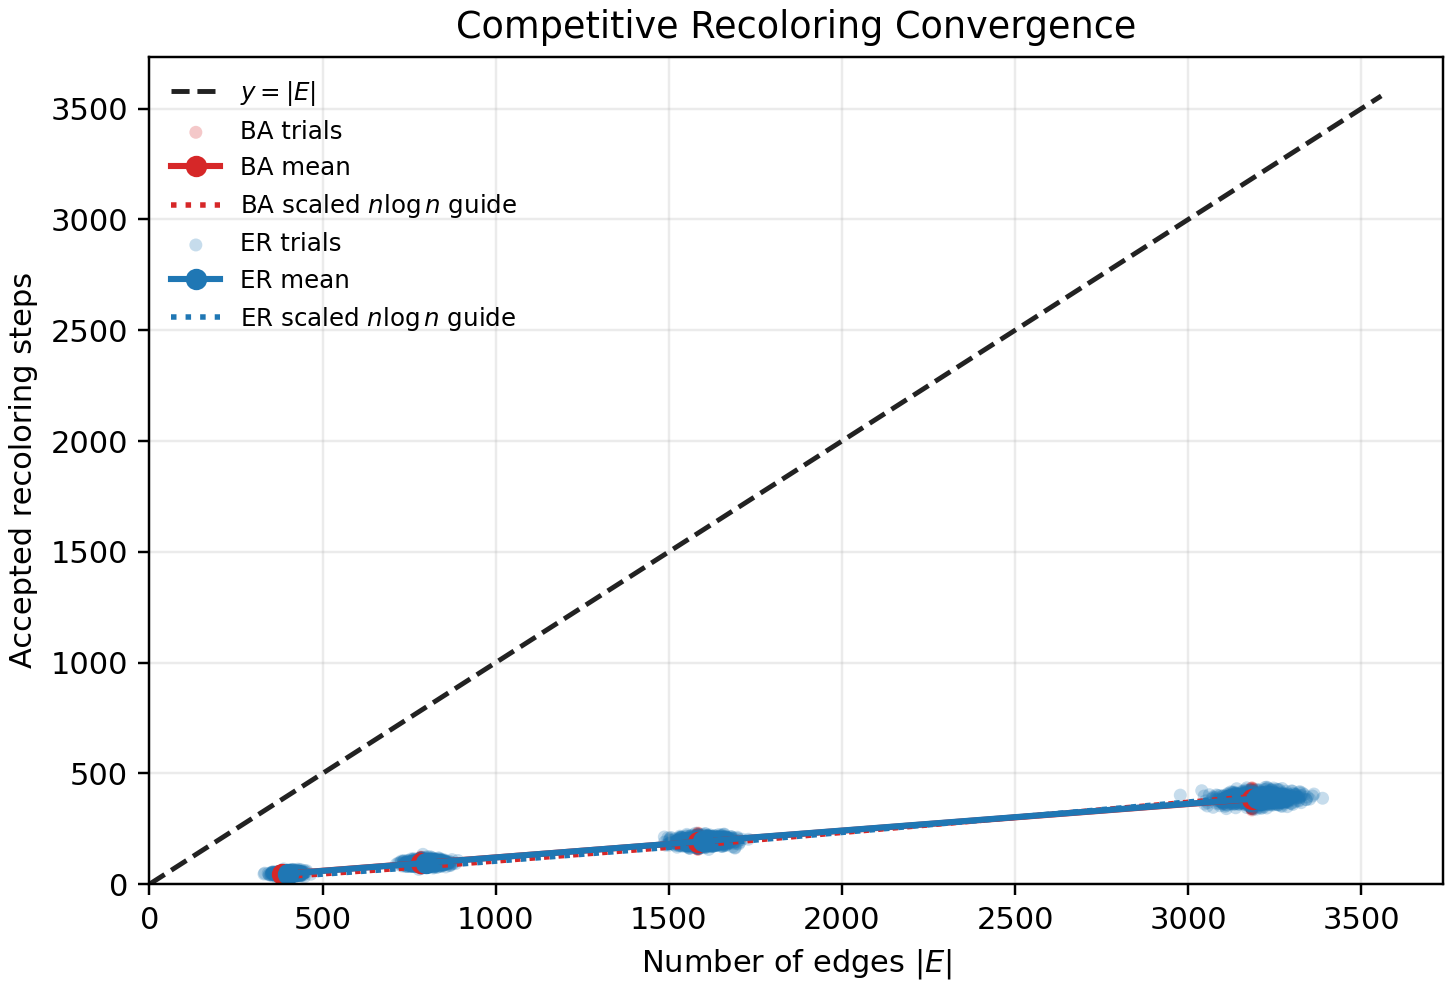
\includegraphics[width=0.92\linewidth]{figures/steps_vs_edges.png}
    \caption{Accepted recoloring steps versus the deterministic edge bound.
    Each point is one trial on a sparse Erd\H{o}s--R\'enyi or
    Barab\'asi--Albert graph. The dashed line is $T=|E|$. The empirical
    trajectories remain far below the worst-case Lyapunov bound.}
    \label{fig:steps-vs-edges}
\end{figure}

\begin{remark}
The observed speedup is consistent with the randomized asynchronous schedule:
activation orders that approach the deterministic worst case are rarely sampled
in standard sparse graph ensembles. The experiments suggest behavior closer to
$\mathcal{O}(|V|\log |V|)$, and nearly linear in the tested range, but the
formal guarantee used here remains the deterministic edge bound in
Theorem~1.
\end{remark}

\section{Conclusion}

Competitive graph recoloring admits an exact discrete Lyapunov function: the
number of monochromatic edges. This yields a concise finite-time convergence
proof and a deterministic accepted-move bound of
$T\le \Phi(c(0))\le |E|$. The simulations confirm the bound and indicate much
faster typical convergence on standard sparse random graph families.

The result is intentionally local: it does not require a central coordinator,
global optimization oracle, or assumptions on the activation order beyond
single-vertex asynchronous updates. Since global minimization of conflicts is
intractable in general, the value of the theorem is to certify that a purely
selfish rule still has a finite, monotone path to equilibrium. This separates
the achievable distributed guarantee from the harder question of finding a
globally optimal coloring, and it explains why the empirical behavior can be
studied cleanly through the same potential.

\paragraph*{Acknowledgements}
The authors thank their mentors, colleagues, and peers for encouragement and
helpful feedback. This research received no external funding. The simulation
code is available from the authors upon reasonable request.

\begin{thebibliography}{99}

\bibitem{nash1951}
J. Nash,
Non-cooperative games,
\textit{Annals of Mathematics} 54 (1951) 286--295.

\bibitem{rosenthal1973}
R. W. Rosenthal,
A class of games possessing pure-strategy Nash equilibria,
\textit{International Journal of Game Theory} 2 (1973) 65--67.

\bibitem{monderer1996}
D. Monderer, L. S. Shapley,
Potential games,
\textit{Games and Economic Behavior} 14 (1996) 124--143.

\bibitem{garey1979}
M. R. Garey, D. S. Johnson,
\textit{Computers and Intractability: A Guide to the Theory of
NP-Completeness},
W. H. Freeman, 1979.

\bibitem{frieze1997}
A. Frieze, M. Jerrum,
Improved approximation algorithms for MAX $k$-CUT and MAX BISECTION,
\textit{Algorithmica} 18 (1997) 67--81.

\bibitem{kuhn2006}
F. Kuhn, R. Wattenhofer,
On the complexity of distributed graph coloring,
in: \textit{Proceedings of the 25th Annual ACM Symposium on Principles of
Distributed Computing}, 2006, pp. 7--15.

\bibitem{panagopoulou2008}
P. N. Panagopoulou, P. G. Spirakis,
A game theoretic approach for efficient graph coloring,
in: \textit{Proceedings of the 19th International Symposium on Algorithms and
Computation}, 2008, pp. 183--195.

\bibitem{hopfield1982}
J. J. Hopfield,
Neural networks and physical systems with emergent collective computational
abilities,
\textit{Proceedings of the National Academy of Sciences} 79 (1982) 2554--2558.

\bibitem{apt2012}
K. R. Apt, S. Simon,
A classification of weakly acyclic games,
in: \textit{Proceedings of the 5th International Symposium on Algorithmic Game
Theory}, 2012, pp. 1--12.

\bibitem{erdos1959}
P. Erd\H{o}s, A. R\'enyi,
On random graphs. I,
\textit{Publicationes Mathematicae} 6 (1959) 290--297.

\bibitem{barabasi1999}
A.-L. Barab\'asi, R. Albert,
Emergence of scaling in random networks,
\textit{Science} 286 (1999) 509--512.

\end{thebibliography}

\end{document}
